
%% CAPÍTULO 1 %%
\chapter{Introducción}

  %% SECCIÓN %%
  \section{Problema}

 Hoy en día los desarrollos de software especializados en apis son complejos, ya que normalmente se realizaban basándose en base a una arquitectura monolítica, la cual es difícil de  mantener y escalar. En la actualidad se observa como las empresas están decantándose por arquitecturas de microservicios, ya que les otorga muchos beneficios como son estandarización, escalabilidad, mantenimiento y agilidad.
La forma de aplicar los microservicios no es difícil, ya que actualmente existen variadas tecnologías y frameworks que permiten su implementación, además los despliegues se pueden realizar utilizando tecnologías basadas en contenedores tales como Docker y Kubernetes, entre otros. 

\hfill

El problema  que actualmente tienen miles de desarrolladores de Chile,  tanto para trabajo, como para proyectos de desarrollo personal, es que deben  consumir APIs de diferentes fuentes públicas.  Esto genera en muchos casos, que deban recurrir uno por uno, a servicios que no poseen una documentación estandarizada acorde a los tiempos de hoy. Para solventar este problema se implementa, mediante una plataforma de APIs centralizada, la cual se encargará de controlar toda la comunicación y seguridad de los micro servicios, que actualmente están esparcidos en la red. De esta manera se reduce la complejidad que se tiene al implementar este tipo de arquitectura, en donde se necesita tener una pasarela de APIs para los desarrolladores del país.

%   \begin{figure}[!htb]
%     \begin{center}
%     	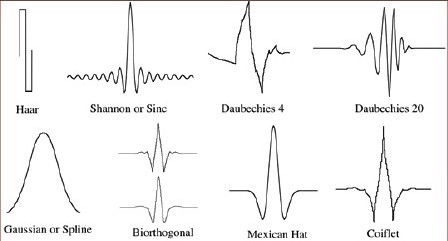
\includegraphics[width=15cm]{./figuras/wavelets.jpg}
%     	\caption{Ejemplos de figura}
%     \end{center}
%     \label{fig:figura}
%   \end{figure}



  %% SECCIÓN %%
  \section{Estado del Arte}
  



